%%%---PREAMBLE---%%%%%%%%%%%%%%%%%%%%%%%%%%%%
\documentclass[oneside,12pt,final]{sty/ucthesis-CA2012}
\pdfoutput=1

%--- Packages ---------------------------------------------------------
\usepackage[lofdepth,lotdepth,caption=false]{subfig}
\usepackage{fancyhdr}
\usepackage{hyperref}
\usepackage{amsmath, amssymb, graphicx}
\usepackage{subfig}
\usepackage{xspace}
\usepackage{braket}
\usepackage{color}
\usepackage{setspace}
\usepackage{tikz}
\usepackage{tikz-3dplot}
\tikzset{>=latex}
%\usepackage{subfigure} (Subfigure package clashes with another package)

%---New Definitions and Commands------------------------------------------------------
\def\p{\partial}
\def\im{\mrm{im}}
\def\Tr{\mrm{Tr}}
\def\Z{\mbb{Z}}
\def\R{\mbb{R}}
\def\C{\mbb{C}}
\def\half{\frac{1}{2}}
\def\filler{\phantom{fillerfillerfiller}}
\newcommand{\be}{\begin{equation}}
\newcommand{\ee}{\end{equation}}
\newcommand{\mbb}[1]{\mathbb{#1}}
\newcommand{\mrm}[1]{\mathrm{#1}}
\newcommand{\mcal}[1]{\mathcal{#1}}
\newcommand{\mbf}[1]{\mathbf{#1}}
\newcommand{\ph}[1]{\phantom{#1}}
\newcommand{\udten}[3]{#1^{#2}_{\ph{#2}#3}}
\newcommand{\duten}[3]{#1^{\ph{#2}#3}_{#2}}
\newcommand{\pd}[2]{\frac{\p#1}{\p#2}}
\newcommand{\D}[2]{\frac{d#1}{d#2}}

%---Set Margins ------------------------------------------------------
\setlength\oddsidemargin{0.25 in} \setlength\evensidemargin{0.25 in} \setlength\textwidth{6.25 in} \setlength\textheight{8.50 in}
\setlength\footskip{0.25 in} \setlength\topmargin{0 in} \setlength\headheight{0.25 in} \setlength\headsep{0.25 in}

%%%---DOCUMENT---%%%%%%%%%%%%%%%%%%%%%%%%%%%%
\begin{document}

%=== Preliminary Pages ============================================
\begin{frontmatter}
	%%%%%%%%%%%%%%%%%%%%%%%%%%%
% TITLE PAGE INFORMATION %
%%%%%%%%%%%%%%%%%%%%%%%%%%%


\title{Simulation of MTD Performance and Measurement of Rare Higgs Decays}

\author{Jonathan Kasuke Guiang}

%%%%%%%%%%%%%%%%%%%%%%%%%%%%%%%%%%
% DECLARATIONS FOR FRONT MATTER %
%%%%%%%%%%%%%%%%%%%%%%%%%%%%%%%%%%
\report{Bachelor's Honors Thesis} \degree{Bachelor of Science} \degreemonth{June} \degreeyear{2019}
\defensemonth{May}
\defenseyear{2019}

\chair{Professor Claudio Campagnari}  % this is your advisor
\othermemberA{Professor David Stuart} % This is a member of your committee 
\othermemberB{Professor Jeffrey Richman} % This is a member of your committee 
\numberofmembers{3} % should match the number of entries above (chair + othermembers)

\field{Physics}
\campus{Santa Barbara}


%\title{{ University of California \\ Santa Barbara} \linebreak \\  Ph.D. Dissertation}
%\author{Tom\'as Andrade}
%\date{2012}

	\maketitle
	\approvalpage
	\copyrightpage
% 	\begin{dedication}

\bigskip

${}$ \\

\bigskip

${}$ \\

\bigskip

${}$ \\

\bigskip

\begin{center}
\begin{Large}
Dedication here
\end{Large}
\end{center}


\end{dedication} 
	\begin{acknowledgements}

The research included in this thesis could not have been performed if not for the assistance, patience, and support of many individuals.  I would first like to extend my deepest gratitude toward my advisor Dr. Claudio Campagnari for his mentorship and constant confidence over the course of my undergraduate studies. It was he who suggested that I study rare Higgs decays, the latter half of this thesis. He also introduced me to Dr. David Stuart, under whose advisement the former half of this thesis was performed. Claudio's support, generosity, and boundless wisdom has made me a better student and physicist.

I would additionally like to thank Dr. David Stuart. His versatile mind and constant effort to encourage learning led me to be more curious and thoughtful. Furthermore, his understanding and amiable treatment of his students promoted a positive environment for learning and practicing physics.

I would also like to extend my appreciation to Dr. Indara Suarez for believing in and guiding me - also to Nick Amin, Bennett Marsh, and Sicheng Wang for your companionship as well as helping me with anything and everything.

This research would not have been possible without the assistance of the CMS experimental collaboration who constructed the experimental apparatus and built the foundations for the data analysis.  

Finally I would like to extend my deepest thanks to my parents Orlando and Cynthia Guiang without whose love, support and understanding I could never have completed this undergraduate degree, nor would I have had the confidence or inspiration to pursue research in physics.

\end{acknowledgements} 
% 	\begin{vitae}
\addcontentsline{toc}{chapter}{Curriculum Vitae}

\begin{vitaesection}{Education}
\vspace{-0.1cm}
\item [2019]	B.S. in Physics (Expected), University of California, Santa Barbara.
\end{vitaesection}

\textbf{Publications}

Publications.

\end{vitae}
	%
%  Abstract
%

\begin{abstract}
\addcontentsline{toc}{chapter}{Abstract}
%todo: max 350 words

Progress in experimental High Energy physics can be derived from efforts in two fundamentally-linked domains: detector design and data analysis. Novel or otherwise improved detector designs push the boundaries of human perception, while rigorous, academically-motivated data analysis furthers the extent of human understanding. Therefore, both pursuits build towards the discovery of new physics, but they cannot be completely effective without the other. As such, this thesis covers them both. First, a simple, yet dynamic and effective simulation of the performance of a proposed addition to the CMS detector for the upcoming HL-LHC upgrade is described. Its programmatic construction allowed for clear and concise answers to challenging design questions posed during the upgrade's conceptual proposal and technical design. Second, a measurement of rare Higgs-boson decays, $H \rightarrow \rho+\gamma$ and $H \rightarrow \phi+ \gamma$, is performed using data based on a sample of proton-proton collisions collected by the Compact Muon Solenoid (CMS) detector at the Large Hadron Colider (LHC). Most notably, a Boosted Decision Tree (BDT) is used for distinguishing signal from background data after showing significant improvement over traditional, cut-based methods. This exploration is motivated by the possibility of measuring anomalous rates of these two particularly rare decay modes, which would reveal the existence of new physics.

%\abstractsignature
\end{abstract}



	\tableofcontents
\end{frontmatter}

\begin{mainmatter}

%---Set Headers and Footers ------------------------------------------------------
\pagestyle{fancy}
\renewcommand{\chaptermark}[1]{\markboth{{\sf #1 \hspace*{\fill} Chapter~\thechapter}}{} }
\renewcommand{\sectionmark}[1]{\markright{ {\sf Section~\thesection \hspace*{\fill} #1 }}}
\fancyhf{}

\makeatletter \if@twoside \fancyhead[LO]{\small \rightmark} \fancyhead[RE]{\small\leftmark} \else \fancyhead[LO]{\small\leftmark}
\fancyhead[RE]{\small\rightmark} \fi

\def\cleardoublepage{\clearpage\if@openright \ifodd\c@page\else
  \hbox{}
  \vspace*{\fill}
  \begin{center}
    This page intentionally left blank
  \end{center}
  \vspace{\fill}
  \thispagestyle{plain}
  \newpage
  \fi \fi}
\makeatother
\fancyfoot[c]{\textrm{\textup{\thepage}}} % page number
\fancyfoot[C]{\thepage}
\renewcommand{\headrulewidth}{0.4pt}

\fancypagestyle{plain} { \fancyhf{} \fancyfoot[C]{\thepage}
\renewcommand{\headrulewidth}{0pt}
\renewcommand{\footrulewidth}{0pt}}

%=== Introduction ============================================
\chapter{Introduction}

Over the last century, the Standard Model (SM) has been shown to be the most accurate description of the fundamental construction and operation of the universe, but it is still incomplete, giving rise to many theories including Supersymmetry (SUSY), a popular extension of the Standard Model. It predicts a partner particle to every SM particle, which would resolve some particularly bothersome issues with the Standard Model like fixing the mass of the Higgs Boson, the identity of Dark Matter, and many others. Assuming SUSY is real, supersymmetric particles are expected to appear in high-energy collisions at the Large Hadron Particle Collider (LHC). However, direct evidence for SUSY, or for any other competing theory, has yet to be discovered, thus motivating the continual development of the LHC and of the field of High Energy physics as a whole. Progress at the LHC is due to two fundamentally connected and absolutely essential aspects of High Energy physics: detector design and data analysis - the detector provides the data, but the analysis makes it useful. As such, developments on both sides of the process offer the potential for finding new physics.

\begin{section}{Permissions and Attributions}
\begin{enumerate}

\item The content of chapter 2 and appendix A is the result of a collaboration with Alice and Bob, and has previously appeared in the (Journal) (paper citation). It is reproduced here with the permission of (Institution): \url{http://}.

\end{enumerate}
\end{section}

%=== Chapter 2  ============================================
\chapter{MTD Simulation}
%
%  MTD Simulation
%

\begin{section}{Motivation}

The HL-LHC upgrade will offer unprecedented luminosity in which one may find new physics, but it brings with it new complications that must be addressed by upgraded or additional detector hardware. Foremost among the new challenges posed by the HL-LHC is that higher luminosity means many more particles, which provides a far more complex picture to reconstruct for analysis. One such complexity is the increase in collision points, which is a key component of both offline and online reconstruction. With more particles colliding, collision points start to ``pile up'' on top of each other in space (this phenomena is aptly referred to as \textit{pileup}). Consequently, when reconstructing collisions into discrete ``events,'' one for each proton-proton collision, the reconstruction algorithm is unable to discern between one collision and many others that occurred in the same point in space. However, these collisions occur at different \textit{times}, so adding timing information should certainly help reduce pileup. In fact, this has been studied and proven to be the case in simulations (Fig. \ref{fig:pileup-reduce}). To this end, it has been proposed that a layer of silicon-based sensors called the MIP Timing Detector (MTD), with sufficient timing resolutions, be placed around the perimeter -- surrounding the barrel and covering the endcap -- of the CMS detector, but the design and approval of such an upgrade is no simple task. From its conceptual inception to the finalization of its technical design, questions continually arise, so clear, cogent answers are constantly required, but since the detector has yet to be built, computer simulations are necessary to address these important concerns regarding the design and projected performance of the MTD.

\begin{figure}[htb]
\begin{center}
\subfloat      {
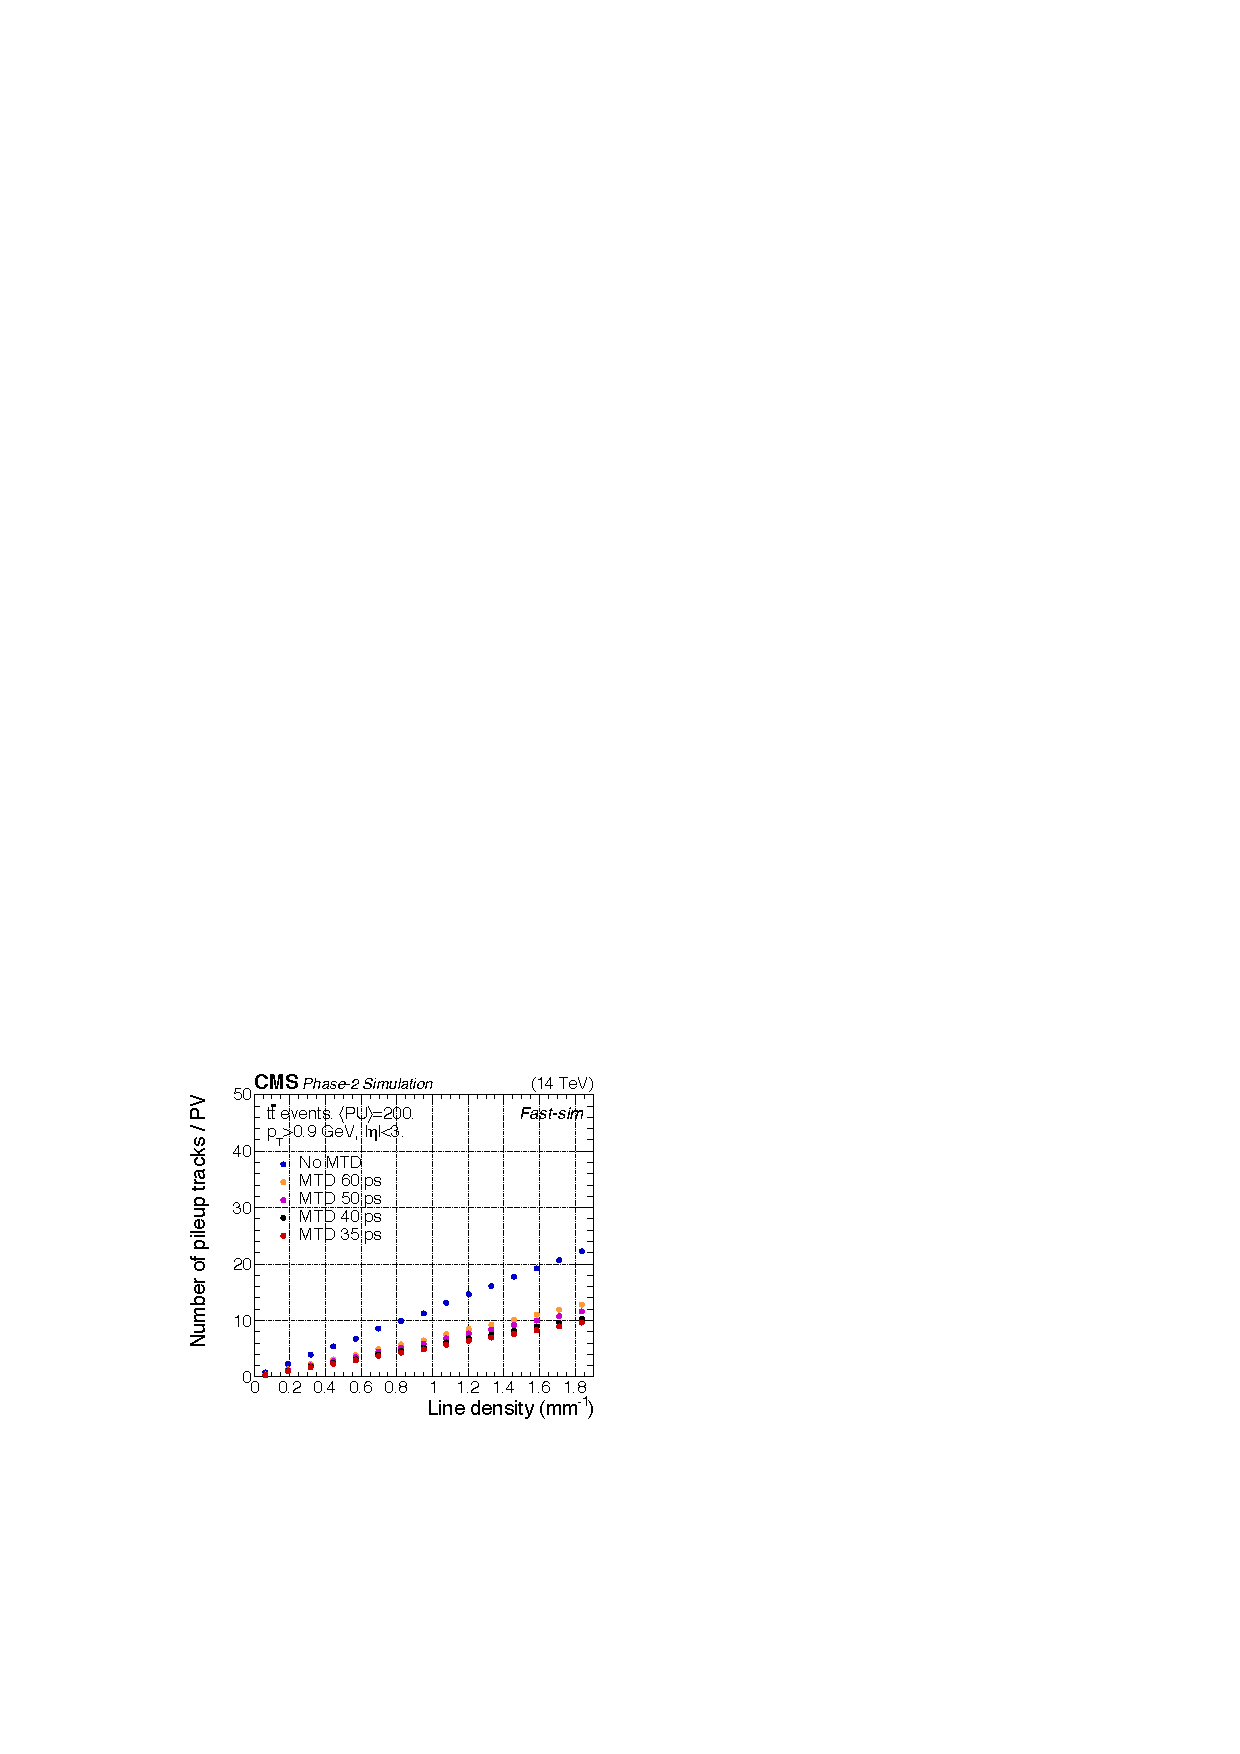
\includegraphics[width=.45\linewidth]{Dissertation/fig/pileup-reduce1.pdf}
}\quad
\subfloat      {
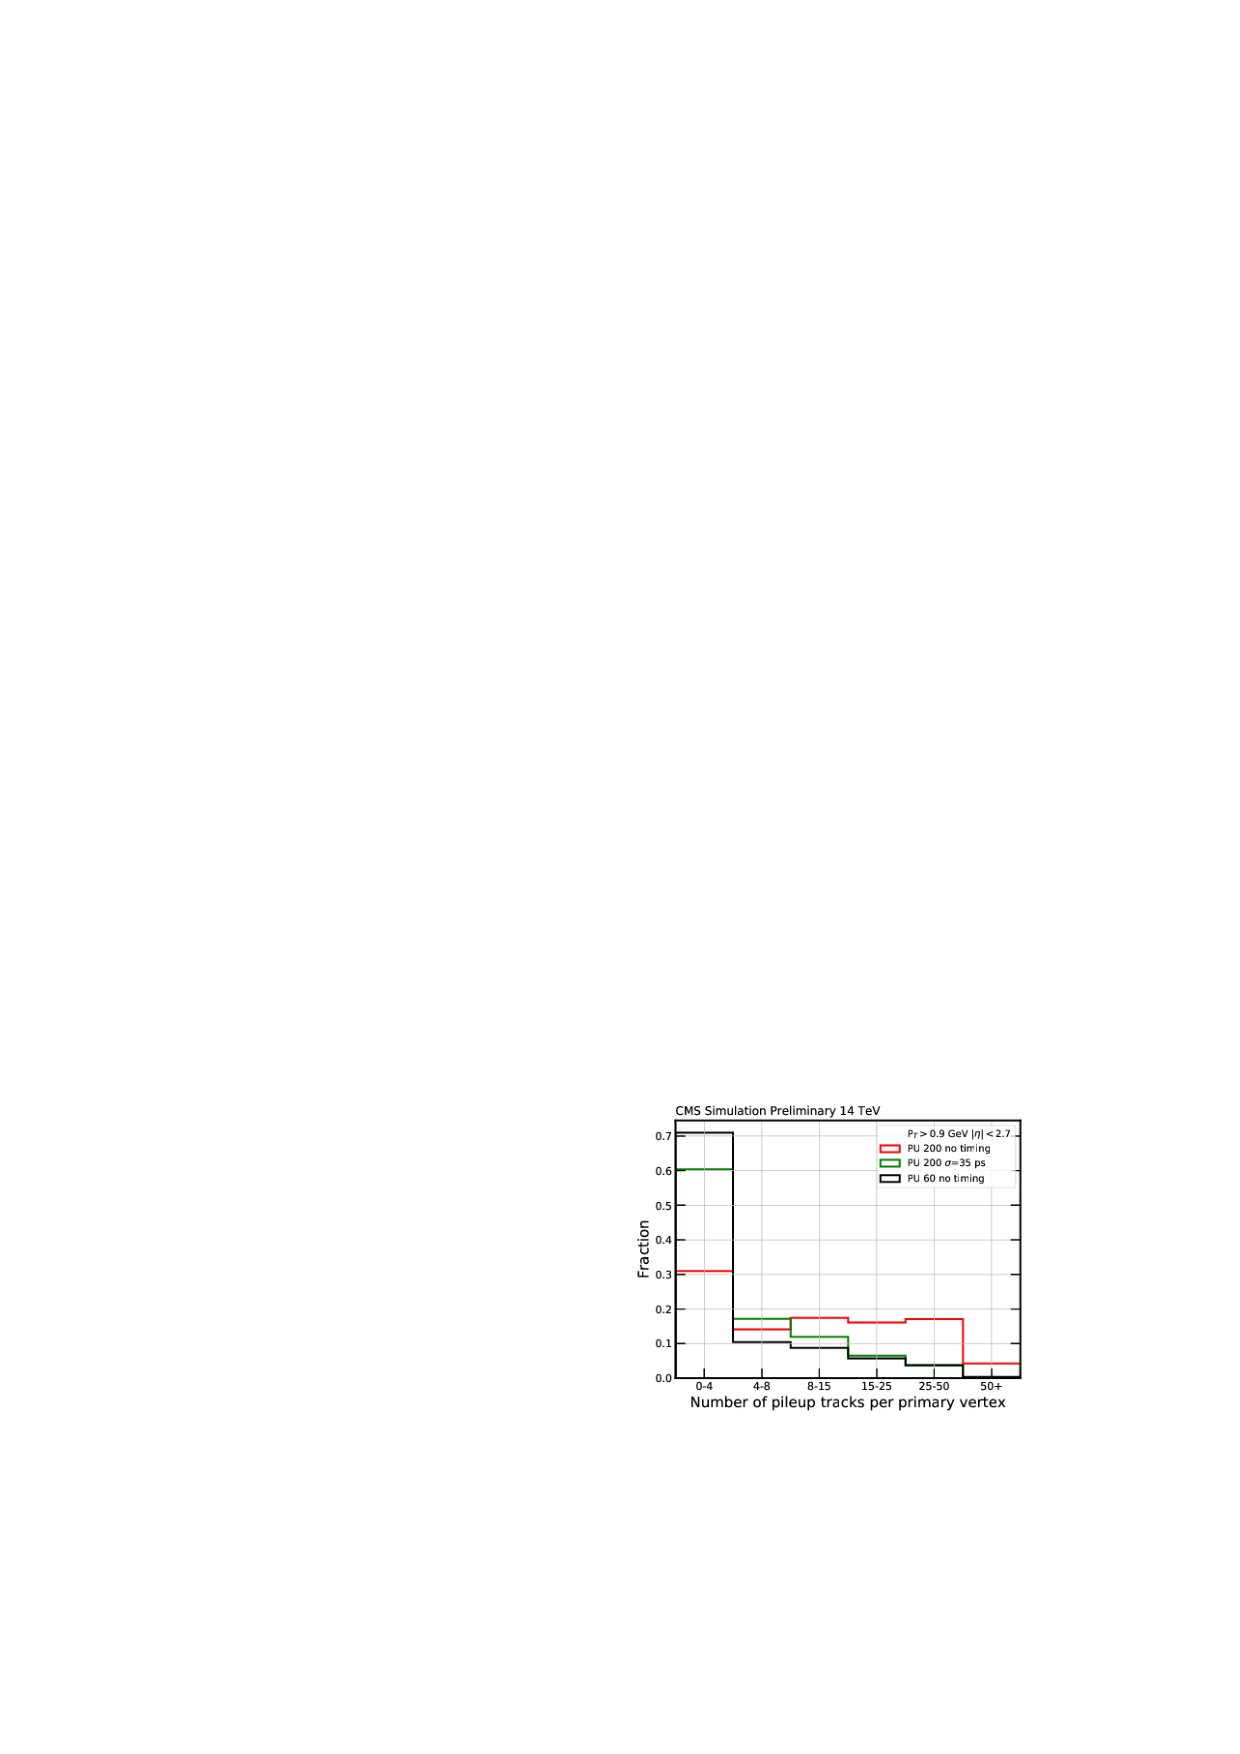
\includegraphics[width=.45\linewidth]{Dissertation/fig/pileup-reduce2.pdf}
}
\end{center}
\caption{Plots from the TDR\cite{cite-mtd-tdr} demonstrating pileup reduction from timing information. Left: Number of pileup tracks incorrectly associated with the hard interaction vertex as a function of the collision line density for different time resolutions. Right: Distribution of the number of incorrectly associated tracks with the use of a $3\sigma$ (where $\sigma = 35$ ps) selection on timing information and without use of timing information; the vertical axis is the fraction of primary vertices which have the number of pileup tracks shown on the horizontal axis
associated to them.}
\label{fig:pileup-reduce}
\end{figure}

\end{section}

\begin{section}{The Topolino Design}

The barrel and endcap layers (BTL and ETL respectively) of the MTD have rotational symmetries -- they are round -- while the sensors are rectangular, so some careful consideration is required when looking to cover the CMS detector with a new sensor layer. For the BTL, the design is fairly simple: long trays of sensors may be laid along the axis of the barrel, maintaining its cylindrical symmetry. However, correctly fitting the rectangular sensors to the circular space allotted on the endcaps (which are essentially annuli) becomes a complicated exercise in geometric optimization, while including space for all of the required circuitry, wiring, and cooling systems imposes complicated physical constraints.  Although the ETL offered unique complications, one design was arrived at -- named ``Topolino'' (Mickey Mouse in Italian) by its inventor -- where the ETL is divided into four ninety-degree wedges. The front of each wedge is tiled with parallel strips of sensors that continue up until the the edge of the endcap. The back of the same wedge is similarly covered, but the sensors are horizontally offset to cover the gaps left by the readout electronics on the front. Each wedge is covered in this way, then placed such that the sensors in each is perpendicular to its neighboring wedges. See Figure \ref{fig:topolino} for a detailed visualization of the proposed design.

\begin{figure}[htb]
\begin{center}
\subfloat[Rendered with no mounting disk to show coverage of electronics gaps.]      {
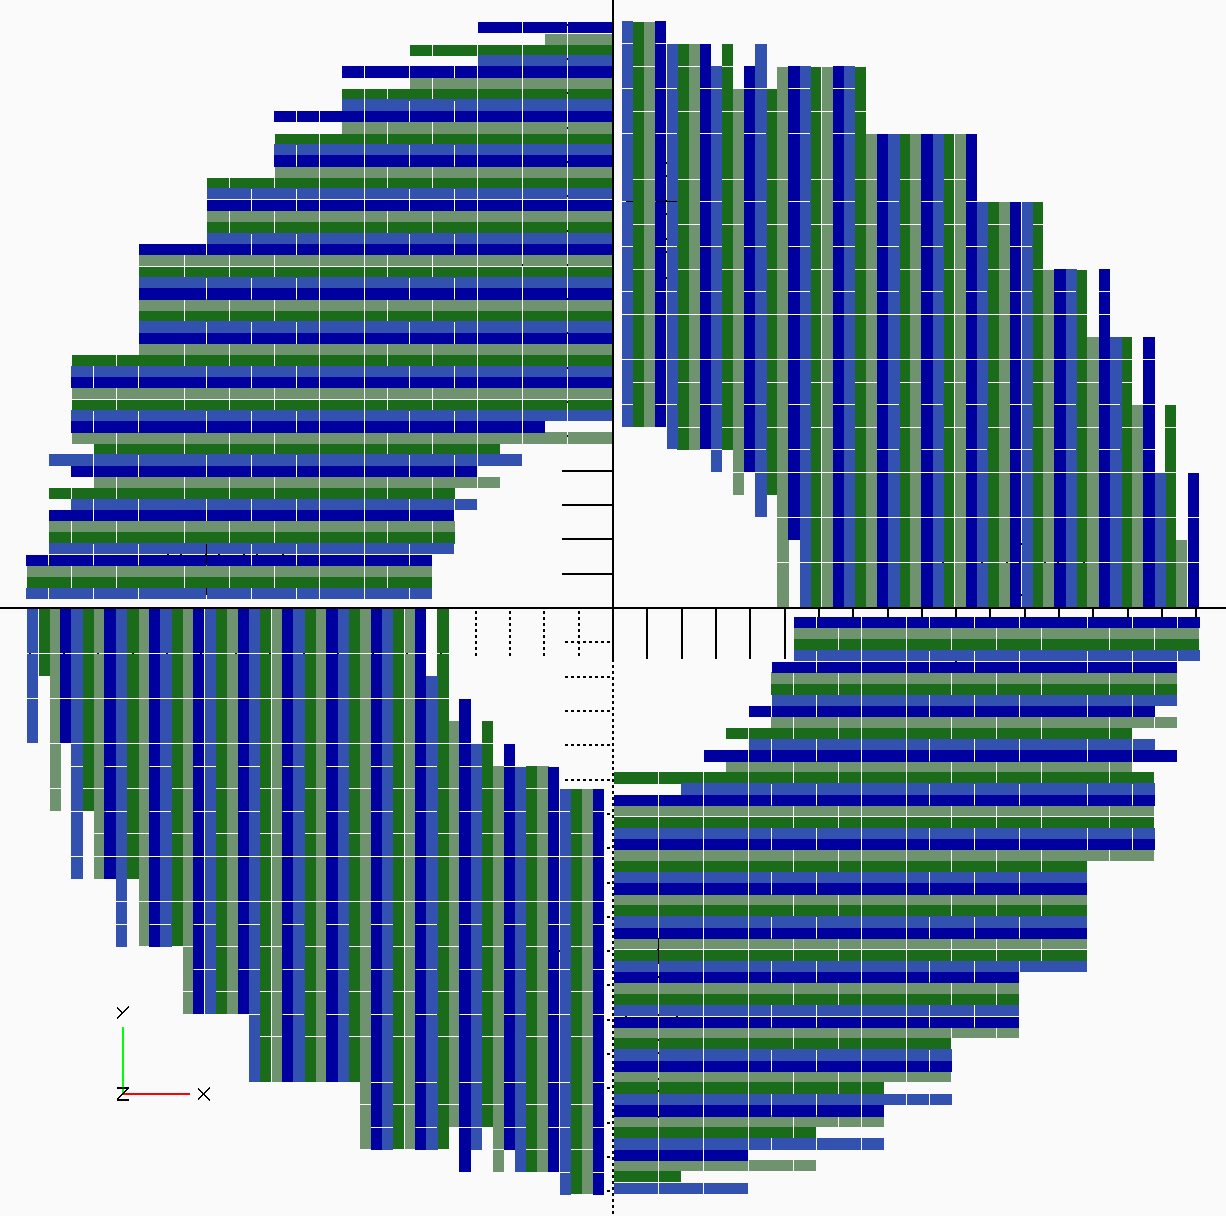
\includegraphics[width=.5\linewidth]{Dissertation/fig/topolino-nodisk.png}
}
\\
\subfloat[Front of one full disk.]      {
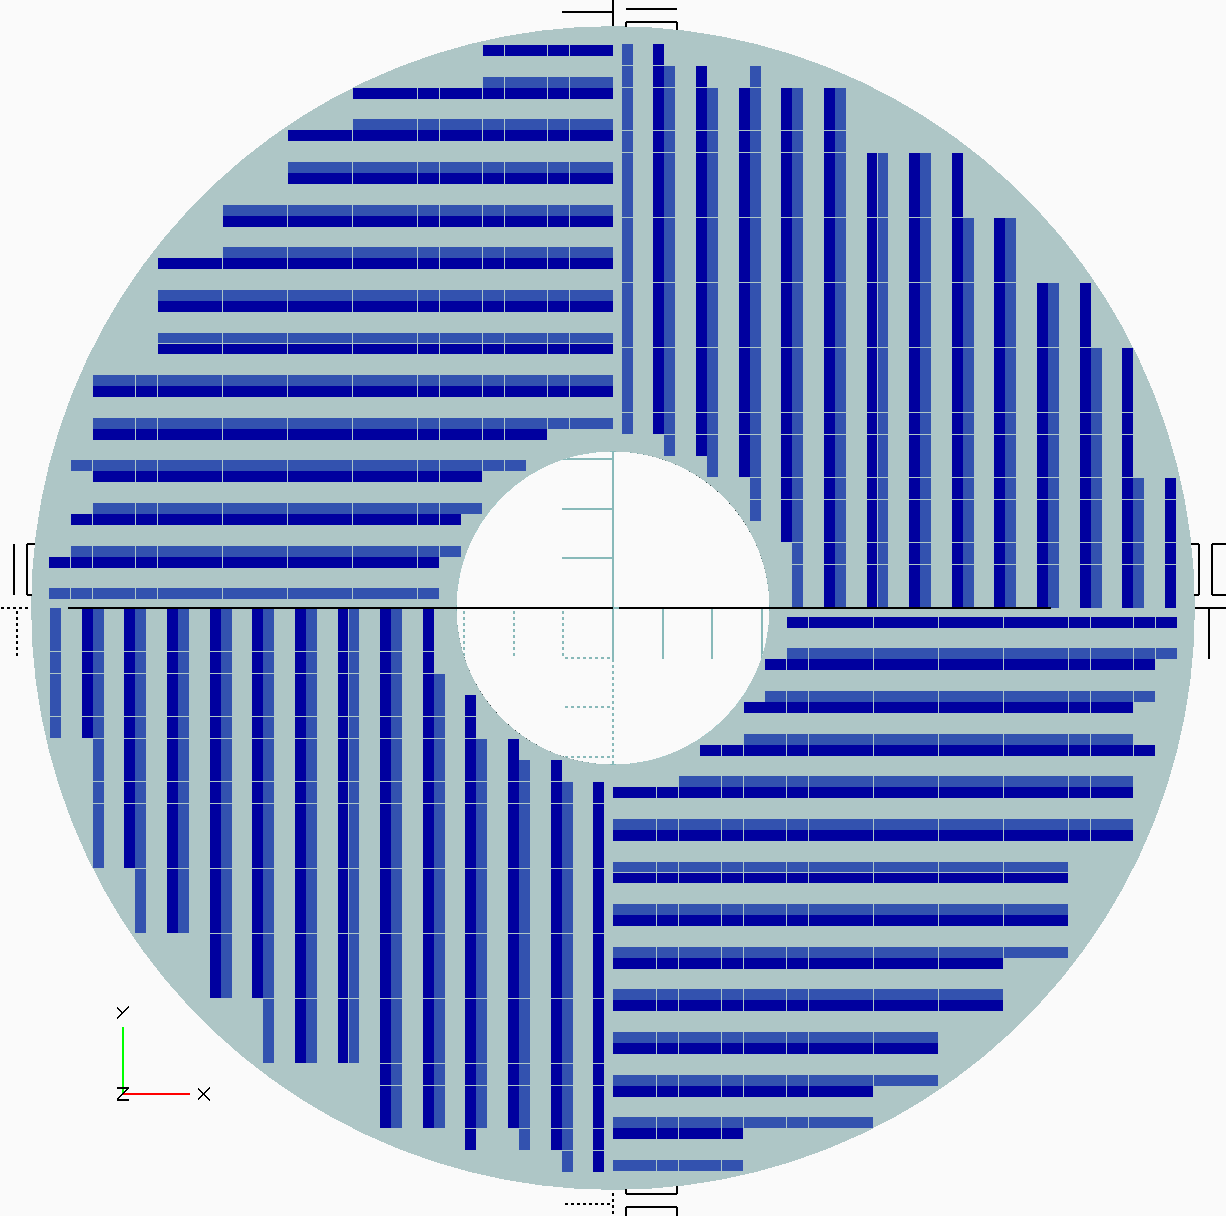
\includegraphics[width=.25\linewidth]{Dissertation/fig/topolino-front.png}
}\quad
\subfloat[Back of one full disk.]      {
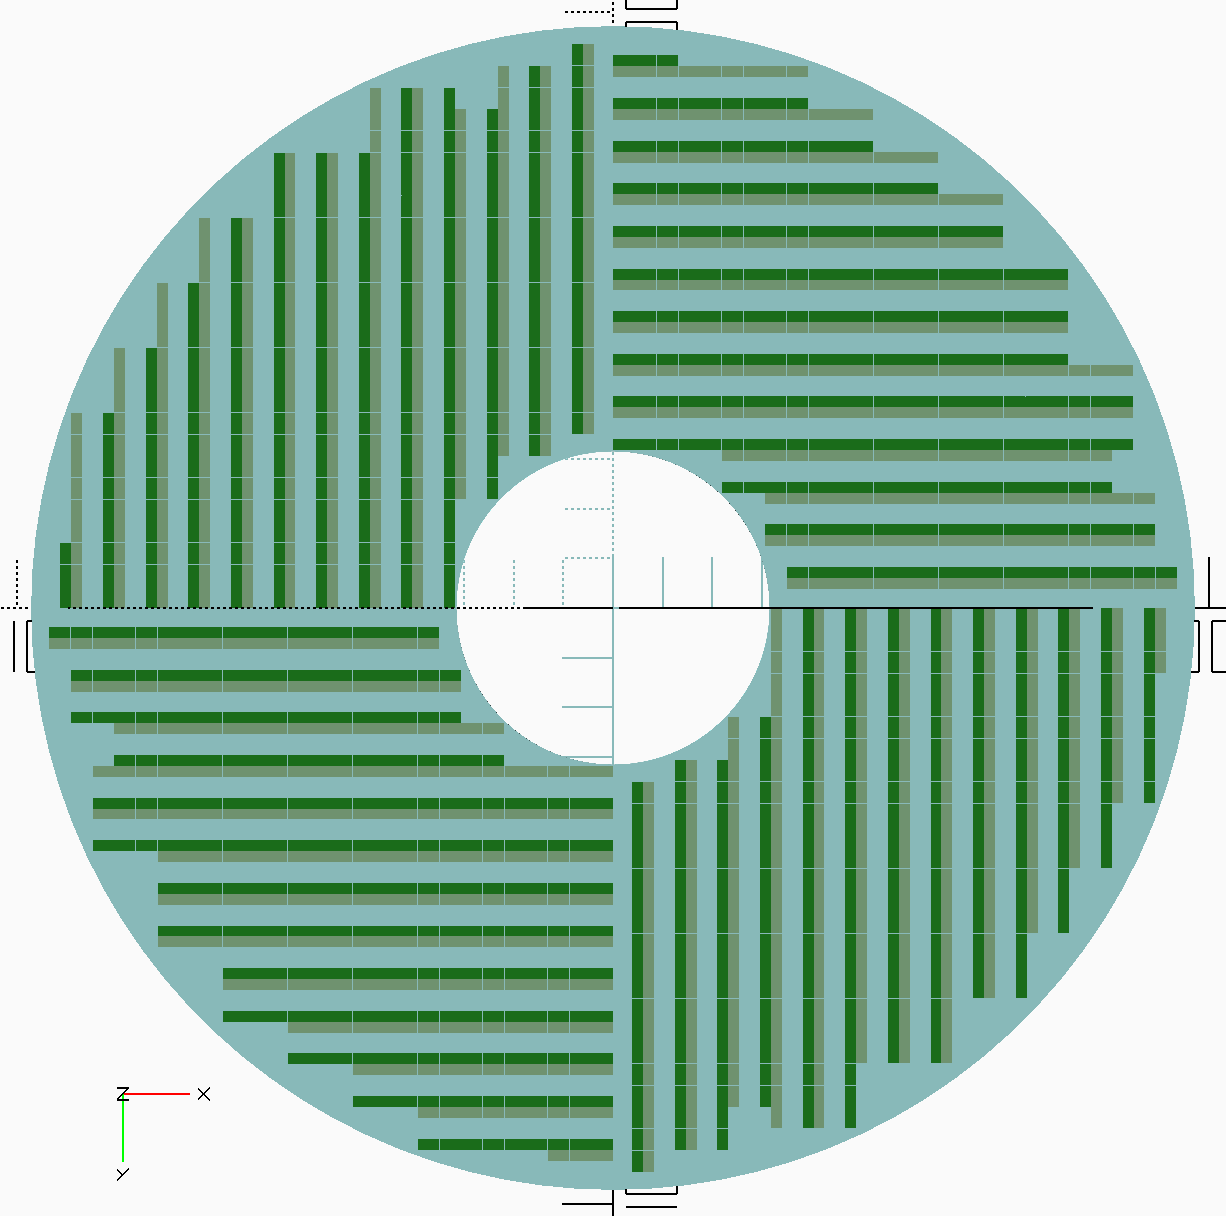
\includegraphics[width=.25\linewidth]{Dissertation/fig/topolino-back.png}
}
\end{center}
\caption{The ``topolino'' design.}
\label{fig:topolino}
\end{figure}

\end{section}

\begin{section}{Rendering the Detector}

Detector physics simulation begins with a simulation of the detector, but for answers to questions about the MTD's design and performance, verbose considerations of minute physical interactions are, at the moment, unnecessary. Therefore, though more complex tools offer more accurate physics, a simple rendering of each sensor's position is space is sufficient. However, the simulation must also be configurable, so assembling the it by hand, like most 3D-modeling software requires, was neither an entertaining, nor efficient solution. Instead, OpenSCAD, a C-like programming language that allows for simple, modular construction of three-dimensional models, was selected.

To algorithmically implement the Topolino design, fundamental rules that govern the layout had to be established. First, neither the sensors, nor the space allotted for their circuitry, could be allowed to hang over the perimeter of the endcap. Second, sensors are most easily assembled and placed as modules, so the detector must be tiled by \textit{groups} of sensors. Finally, the service modules -- the ``circuitry'' for which space has already been allotted -- are designed to service sensors on both sides, so sensors should (generally) be placed as such, resulting in a neat grid. With these rules in mind, an algorithm parses the x-axis in increments equal to the width of a sensor module, then places sensors by their lower, left-hand (closest to origin) corners, so long as their placement does not violate any of the previously stated rules. One wedge is tiled in this way where the sensors on its reverse side are placed in the same way but starting from a given displacement from the origin such that the holes left by the spacing for readout electronics are covered by sensors on the opposite side. The rest of the endcap is covered by simply taking this wedge, then placing orthogonally-rotated copies until the entire surface is covered. The images shown in Figure \ref{fig:topolino} were created by the algorithm described here.

\end{section}

\begin{section}{Simulating Performance}
\begin{subsection}{Pre-processing}
The three-dimensional model of the MTD can be exported as a Standard Tessellation Language (STL) file. During the export process, each independent object -- say, a single sensor which is represented as a thin rectangular prism -- is broken down into each of its constituent faces. Then, it undergoes the tessellation process, wherein the face considered is broken into some optimal number of constituent triangles (hereafter referred to as \textit{polygons}). The \textit{vertices} of each of these polygons are then written to the STL file, in a clockwise order relative to the origin. It is important to note that this guarantees that the \textit{facet normal} vector -- that is, a vector orthogonal to the surface of the polygon with a magnitude equal to the area of the polygon -- always points outwards with respect to the origin.
\end{subsection}
\begin{subsection}{Hit Detection Algorithm}
Now, before the simulation itself is generally discussed, the algorithm by which an intersection between a point and a polygon is determined should first be outlined, since it is the core operation of the simulation but is otherwise only tangentially important to the overall process. Consider a triangle in three-space, namely a set of three vectors $\vec{v}_1, \vec{v}_2, \vec{v}_3$ with facet normal $\hat{n}$, normalized such that $|\hat{n}| = 1$, pointing outwards relative to the origin. Then, suppose there exists a point $\vec{a}$ somewhere in three-space (see Figure \ref{fig:setup} for a visual representation of this setup). First, the coordinate system must be rotated into the plane of the polygon (in order to account for both the azimuthal symmetry of the BTL and radial symmetry of the ETL). One basis vector, arbitrarily chosen to be $\hat{e}_3'$, is already given by the facet normal vector. Another, now chosen to be $\hat{e}_{1}'$, is given by the original $\hat{e}_3$ vector (this is $\hat{z}$ is the CMS coordinate system; see Appendix \ref{appendix:cms-coords} for more information). With two basis vectors determined, the third is simply given by the cross product $\hat{e}_3'\times\hat{e}_1'$, assuming they are already normalized (again, see Figure \ref{fig:setup}). From this new set of basis vectors $\hat{e}_i'$, still represented in the original basis, a matrix $R$ can be constructed to translate any arbitrary vector into the primed coordinate system:

\begin{equation}
    \hat{e}_i' = \begin{pmatrix} x_i \\ y_i \\ z_i \end{pmatrix}
    \rightarrow
    R \equiv \begin{pmatrix} 
        x_1 & y_1 & z_1 \\
        x_2 & y_2 & z_2 \\
        x_3 & y_3 & z_3
    \end{pmatrix}
\end{equation}

\noindent The point $\vec{a}$ and vertices $\vec{v}_i$ are translated into the primed coordinate system such that $R\vec{a} = \vec{a}'$ and $R\vec{v}_i = \vec{v}_{i}'$. Then, the $\hat{e}_3'$ coordinates of $\vec{a}'$ and $\vec{v}_i'$ are set to zero, ensuring that all points considered are in the same plane parallel to that spanned by the polygon. Now, the vector from the point $\vec{a}'$ to the vertex $\vec{v}_{i}'$ is defined as $\vec{d}_{i}' \equiv \vec{v}_{i}'-\vec{a}'$. Finally, the following cross products are defined:

\begin{equation}
    \vec{C}_{i}' \equiv \epsilon_{ijk}(\vec{d}_{j}'\times\vec{d}_{k}')
\end{equation}

\noindent In words, the vectors $\vec{C}_{i}'$ are the cross products between adjacent vectors $\vec{d}_{j}'$, $\vec{d}_{k}'$ taken in cyclical permutations, as dictated by the Levi-Cevita symbol $\epsilon_{ijk}$. More importantly, however, each vector $\vec{C}_{i}'$ must be \textit{parallel} to the facet normal vector, which is $\hat{e}_{3}'$ in the primed coordinate system, if the point $\vec{a}$ lies \textit{inside} of the polygon. This is because the angles between each vector $\vec{d}_{i}'$ must add up to 180 degrees inside the polygon or 360 degrees outside by geometric constraint, so the angle between two vectors $\vec{d}_{i}'$, $\vec{d}_{j}'$ has an upper limit of 180 degrees inside of the triangle and 360 degrees outside. Thus, the cross product between these vectors will point one way (here, the positive $\hat{e}_3'$ direction) if the angle between them is less than 180 degrees or exactly anti-parallel (the $-\hat{e}_3'$ direction) otherwise, so if all $\vec{C}_{i}'$ are greater than zero, $\vec{a}$ must be inside of the polygon, otherwise, it can immediately determined that $\vec{a}$ is outside. Put concisely, point $\vec{a}$ intersects the polygon given by $\vec{v}_1, \vec{v}_2, \vec{v}_3$ and facet normal $\hat{n}$ if and only if $\vec{C}_{i}' > 0$ where $i\in[1,2,3]$.

\begin{figure}[htb]
\begin{center}

\subfloat[Original]      {
\tdplotsetmaincoords{60}{110}
\begin{tikzpicture}[scale=3,tdplot_main_coords]
 
  % variables
  % theta, phi for a
  \def\rvec{.8}
  \def\thetavec{30}
  \def\phivec{345}
  % theta, phi for v1
  \def\rvecone{1.0}
  \def\thetavecone{15}
  \def\phivecone{90}
  % theta, phi for v2
  \def\rvectwo{1.0}
  \def\thetavectwo{74}
  \def\phivectwo{54}
  % theta, phi for v3
  \def\rvecthree{0.8}
  \def\thetavecthree{74}
  \def\phivecthree{90}
  % theta, phi for n
  \def\rvecfour{.7}
  \def\thetavecfour{37}
  \def\phivecfour{72}
 
  % axes
  \coordinate (O) at (0,0,0);
  \draw[thick,->] (0,0,0) -- (1,0,0) node[anchor=north east]{$\hat{e}_1$};
  \draw[thick,->] (0,0,0) -- (0,1,0) node[anchor=north west]{$\hat{e}_2$};
  \draw[thick,->] (0,0,0) -- (0,0,1) node[anchor=south]{$\hat{e}_3$};
 
  % a
  \tdplotsetcoord{P}{\rvec}{\thetavec}{\phivec}
  \draw[-stealth,black] (O)  -- (P) node[above right] {$\vec{a}$};
  \draw[dashed,black]   (O)  -- (Pxy);
  \draw[dashed,black]   (P)  -- (Pxy);
  % n
  \tdplotsetcoord{N}{\rvecfour}{\thetavecfour}{\phivecfour}
  \draw[-stealth,black] (O)  -- (N) node[above right] {$\hat{n}$};
  \draw[dashed,black]   (O)  -- (Nxy);
  \draw[dashed,black]   (N)  -- (Nxy);
  % v1
  \tdplotsetcoord{A}{\rvecone}{\thetavecone}{\phivecone}
  \draw[-stealth,red] (O)  -- (A) node[above right] {$\vec{v}_1$};
  \draw[dashed,red]   (O)  -- (Axy);
  \draw[dashed,red]   (A)  -- (Axy);
  \draw[dashed,red]   (Ay) -- (Axy);
  % v2
  \tdplotsetcoord{B}{\rvectwo}{\thetavectwo}{\phivectwo}
  \draw[-stealth,green] (O)  -- (B) node[above right] {$\vec{v}_2$};
  \draw[dashed,green]   (O)  -- (Bxy);
  \draw[dashed,green]   (B)  -- (Bxy);
  \draw[dashed,green]   (By) -- (Bxy);
  % v3
  \tdplotsetcoord{C}{\rvecthree}{\thetavecthree}{\phivecthree}
  \draw[-stealth,blue] (O)  -- (C) node[above right] {$\vec{v}_3$};
  \draw[dashed,blue]   (O)  -- (Cxy);
  \draw[dashed,blue]   (C)  -- (Cxy);
  \draw[dashed,blue]   (Cy) -- (Cxy);
 
\end{tikzpicture}
}\quad
\subfloat[Primed]      {
\tdplotsetmaincoords{60}{110}
\begin{tikzpicture}[scale=3,tdplot_main_coords]
 
  % variables
  % theta, phi for a
  \def\rvec{.8}
  \def\thetavec{30}
  \def\phivec{345}
  % theta, phi for v1
  \def\rvecone{1.0}
  \def\thetavecone{15}
  \def\phivecone{90}
  % theta, phi for v2
  \def\rvectwo{1.0}
  \def\thetavectwo{74}
  \def\phivectwo{54}
  % theta, phi for v3
  \def\rvecthree{0.8}
  \def\thetavecthree{74}
  \def\phivecthree{90}
  % theta, phi for n
  \def\rvecfour{.7}
  \def\thetavecfour{37}
  \def\phivecfour{72}
  % theta, phi for e2
  \def\rvecfive{1.0}
  \def\thetavecfive{-53}
  \def\phivecfive{90}
 
  % axes
  \coordinate (O) at (0,0,0);
  \draw[thick,->] (0,0,0) -- (1,0,0) node[anchor=north east]{$\hat{e}_{1}'$};
  \tdplotsetcoord{E}{\rvecfive}{\thetavecfive}{\phivecfive}
  \draw[thick,->] (0,0,0) -- (E) node[anchor=north west]{$\hat{e}_{2}'$};
  \tdplotsetcoord{E}{\rvecfour}{\thetavecfour}{\phivecfour}
  \draw[thick,->] (0,0,0) -- (E) node[anchor=south]{$\hat{e}_{3}'$};
 
  % a
  \tdplotsetcoord{P}{\rvec}{\thetavec}{\phivec}
  \draw[-stealth,black] (O)  -- (P) node[above right] {$\vec{a}$};
  \draw[dashed,black]   (O)  -- (Pxy);
  \draw[dashed,black]   (P)  -- (Pxy);
  % v1
  \tdplotsetcoord{A}{\rvecone}{\thetavecone}{\phivecone}
  \draw[-stealth,red] (O)  -- (A) node[above right] {$\vec{v}_1$};
  \draw[dashed,red]   (O)  -- (Axy);
  \draw[dashed,red]   (A)  -- (Axy);
  \draw[dashed,red]   (Ay) -- (Axy);
  % v2
  \tdplotsetcoord{B}{\rvectwo}{\thetavectwo}{\phivectwo}
  \draw[-stealth,green] (O)  -- (B) node[above right] {$\vec{v}_2$};
  \draw[dashed,green]   (O)  -- (Bxy);
  \draw[dashed,green]   (B)  -- (Bxy);
  \draw[dashed,green]   (By) -- (Bxy);
  % v3
  \tdplotsetcoord{C}{\rvecthree}{\thetavecthree}{\phivecthree}
  \draw[-stealth,blue] (O)  -- (C) node[above right] {$\vec{v}_3$};
  \draw[dashed,blue]   (O)  -- (Cxy);
  \draw[dashed,blue]   (C)  -- (Cxy);
  \draw[dashed,blue]   (Cy) -- (Cxy);
 
\end{tikzpicture}
}

\end{center}
\caption{Coordinate systems used.}
\label{fig:setup}
\end{figure}

\begin{figure}[htb]
\begin{center}

\subfloat[Inside]      {
\tdplotsetmaincoords{60}{110}
\begin{tikzpicture}[scale=3,tdplot_main_coords]
 
  % variables
  % theta, phi for v1
  \def\rvecone{1.0}
  \def\thetavecone{90}
  \def\phivecone{90}
  % theta, phi for v2
  \def\rvectwo{1.0}
  \def\thetavectwo{90}
  \def\phivectwo{54}
  % theta, phi for v3
  \def\rvecthree{0.8}
  \def\thetavecthree{90}
  \def\phivecthree{270}
 
  % axes
  \coordinate (O) at (0.2,-0.3,0);
  \draw[thick,->] (0,0,0) -- (1,0,0) node[anchor=north east]{$\hat{e}_1'$};
  \draw[thick,->] (0,0,0) -- (0,1,0) node[anchor=north west]{$\hat{e}_2'$};
  \draw[thick,->] (0,0,0) -- (0,0,1) node[anchor=south]{$\hat{e}_3'$};

  \draw plot [mark=*, mark size=0.5] coordinates{(0.2,-0.3,0)};
  % a
  \draw[-stealth,black] (0,0,0) -- (0.2,-0.3,0) node[above right]{$\vec{a}'$};
  % d1
  \tdplotsetcoord{A}{\rvecone}{\thetavecone}{\phivecone}
  \draw[-stealth,red] (O)  -- (A) node[above right] {$\vec{d}_{1}'$};
  % d2
  \tdplotsetcoord{B}{\rvectwo}{\thetavectwo}{\phivectwo}
  \draw[-stealth,green] (O)  -- (B) node[above right] {$\vec{d}_{2}'$};
  % d3
  \tdplotsetcoord{C}{\rvecthree}{\thetavecthree}{\phivecthree}
  \draw[-stealth,blue] (O)  -- (C) node[above right] {$\vec{d}_{3}'$};
  % d3->d1
  \tdplotdrawarc[thick,->]{(O)}{0.4}{246}{99}
  {anchor=north}{};
  % d1->d2
  \tdplotdrawarc[thick,->]{(O)}{0.4}{99}{68}
  {anchor=north}{};
  % d2->d3
  \tdplotdrawarc[thick,->]{(O)}{0.4}{68}{-114}
  {anchor=north}{};
 
\end{tikzpicture}
}\quad
\subfloat[Outside]      {
\tdplotsetmaincoords{60}{110}
\begin{tikzpicture}[scale=3,tdplot_main_coords]
 
  % variables
  % theta, phi for v1
  \def\rvecone{1.0}
  \def\thetavecone{90}
  \def\phivecone{90}
  % theta, phi for v2
  \def\rvectwo{1.0}
  \def\thetavectwo{90}
  \def\phivectwo{54}
  % theta, phi for v3
  \def\rvecthree{0.8}
  \def\thetavecthree{90}
  \def\phivecthree{270}
 
  % axes
  \coordinate (O) at (-0.75,0,0);
  \draw[thick,->] (0,0,0) -- (1,0,0) node[anchor=north east]{$\hat{e}_1'$};
  \draw[thick,->] (0,0,0) -- (0,1,0) node[anchor=north west]{$\hat{e}_2'$};
  \draw[thick,->] (0,0,0) -- (0,0,1) node[anchor=south]{$\hat{e}_3'$};

  \draw plot [mark=x, mark size=1] coordinates{(-0.75,0,0)};
  % a
  \draw[-stealth,black] (0,0,0) -- (-0.75,0,0) node[above right]{$\vec{a}'$};
  % d1
  \tdplotsetcoord{A}{\rvecone}{\thetavecone}{\phivecone}
  \draw[-stealth,red] (O)  -- (A) node[above right] {$\vec{d}_{1}'$};
  % d2
  \tdplotsetcoord{B}{\rvectwo}{\thetavectwo}{\phivectwo}
  \draw[-stealth,green] (O)  -- (B) node[above right] {$\vec{d}_{2}'$};
  % d3
  \tdplotsetcoord{C}{\rvecthree}{\thetavecthree}{\phivecthree}
  \draw[-stealth,blue] (O)  -- (C) node[above right] {$\vec{d}_{3}'$};
  % d3->d1
  \tdplotdrawarc[thick,->,dashed]{(O)}{0.5}{311}{54}
  {anchor=north}{};
  % d1->d2
  \tdplotdrawarc[thick,->]{(O)}{0.5}{54}{30}
  {anchor=north}{};
  % d2->d3
  \tdplotdrawarc[thick,->]{(O)}{0.5}{30}{-51}
  {anchor=north}{};
 
\end{tikzpicture}
}

\end{center}
\caption{Illustration of vectors from hit position to vertices.}
\label{fig:vectors}
\end{figure}

\end{subsection}
\begin{subsection}{Post-processing}
The STL representation of the MTD and a text file containing the kinematics of many thousands of simulated particle trajectories is now input to a Python program that operates as follows: for each trajectory in the trajectory file, parse over every polygon in the STL file and check if the trajectory intersects the polygon using the algorithm described previously; if intersection, save some kinematics of the trajectory including the hit position; else, continue. This is, in essence, how many ``ray tracing'' algorithms function\cite{raytrace}, which calculate effects like lighting for computer graphics. Ray tracing is a slow process, which is why graphics seen in movies are pre-rendered and far more detailed and realistic than graphics computed in real time, though recent developments are making real-time, brute-force ray tracing more feasible. However, such technology was neither present nor necessary for this simulation. Instead, the Condor\cite{condor} system on the Tier 2 computing center at UC San Diego was used to run the algorithm over approximately 250,000 trajectories. As a result, plots accurate up to the millimeter scale may be produced to study the efficiency of the entire MTD for a dynamic range of geometries. An example of the simulation's output is shown in Figure \ref{fig:chronoplots}.

\begin{figure}[htb]
\begin{center}
\subfloat[]      {
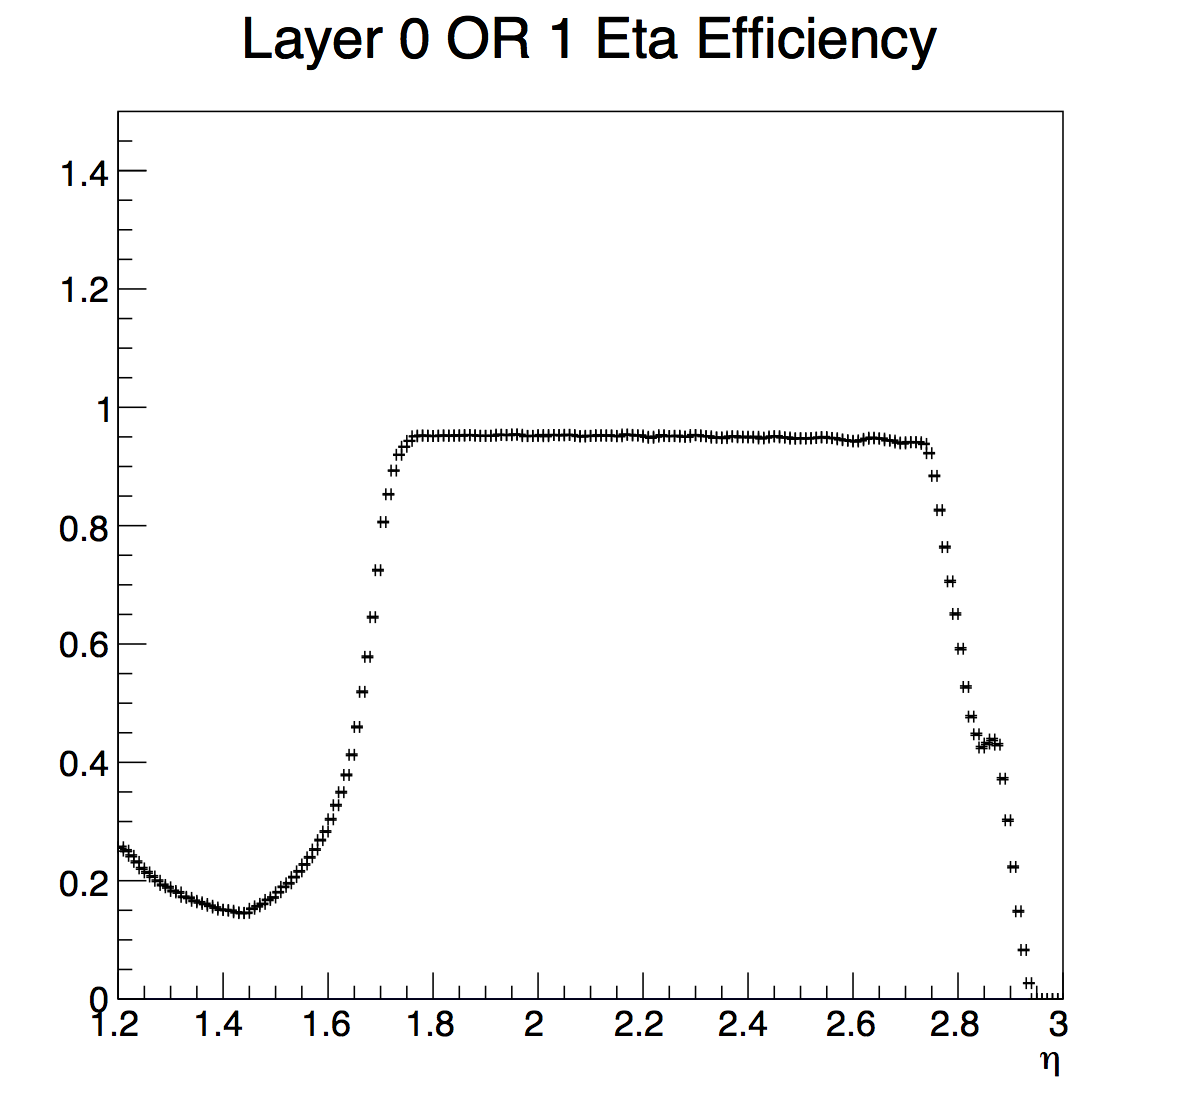
\includegraphics[width=.25\linewidth]{Dissertation/fig/DiskEtaEff01-1190mm.png}
}\quad
\subfloat[]      {
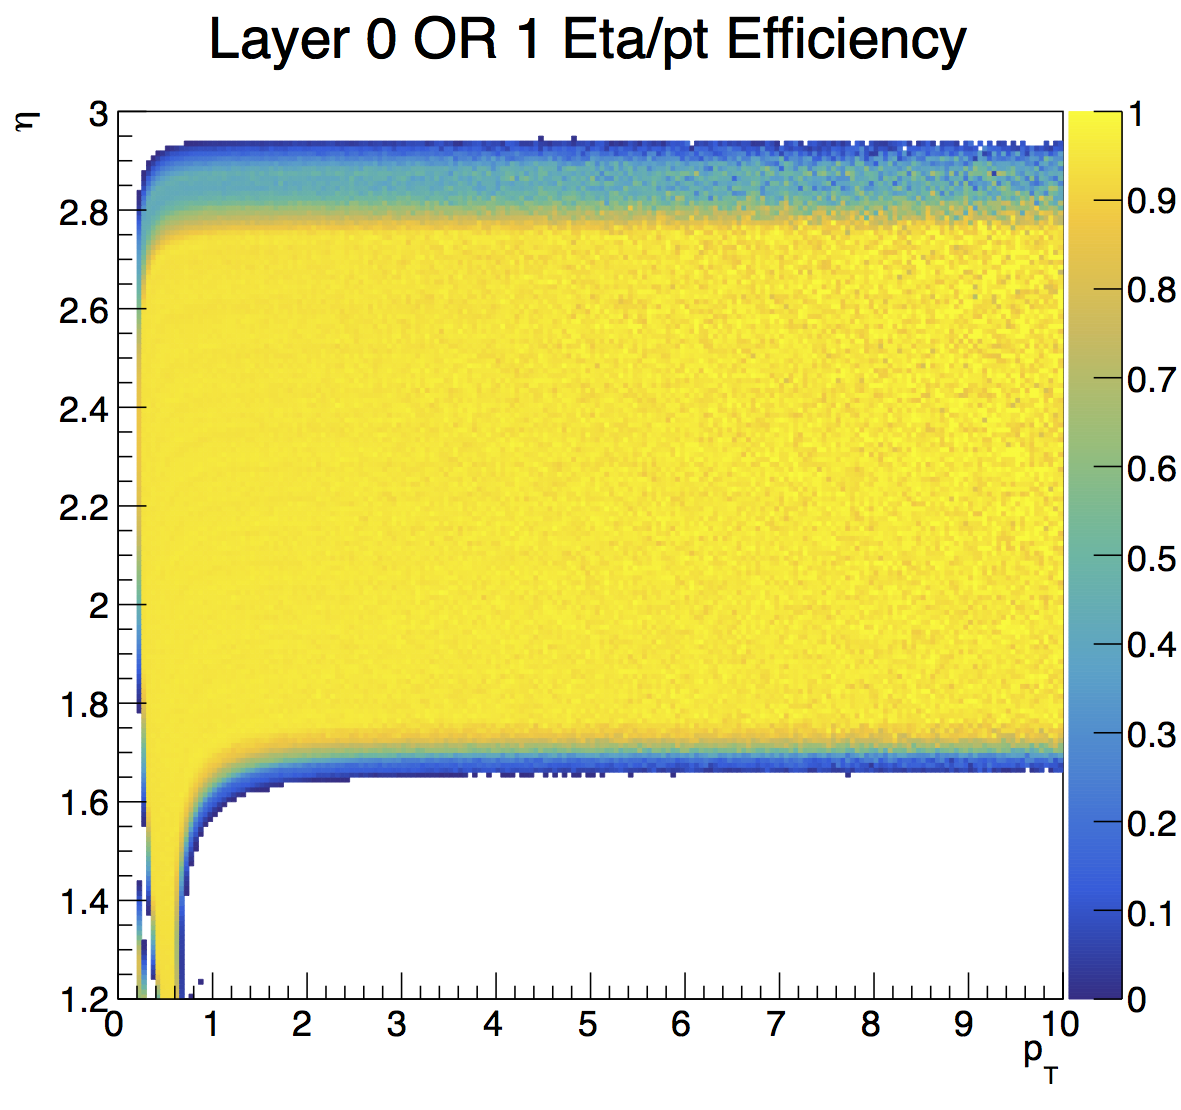
\includegraphics[width=.25\linewidth]{Dissertation/fig/DiskEtaPtEff01-1190mm.png}
}\\
\subfloat[]      {
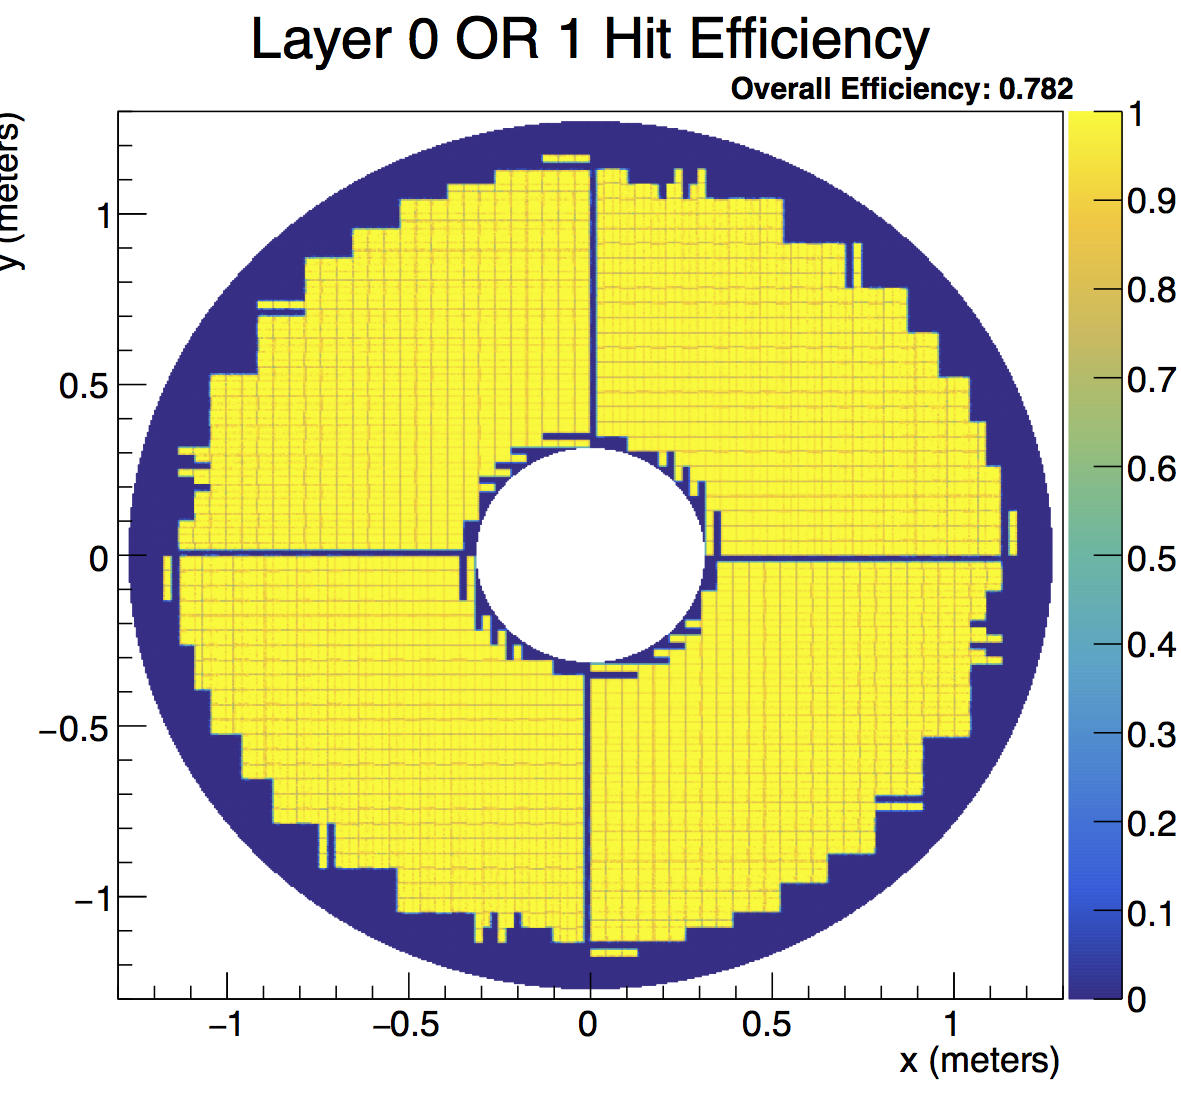
\includegraphics[width=.25\linewidth]{Dissertation/fig/LayerHitEff01-1190mm.png}
}\quad
\subfloat[]      {
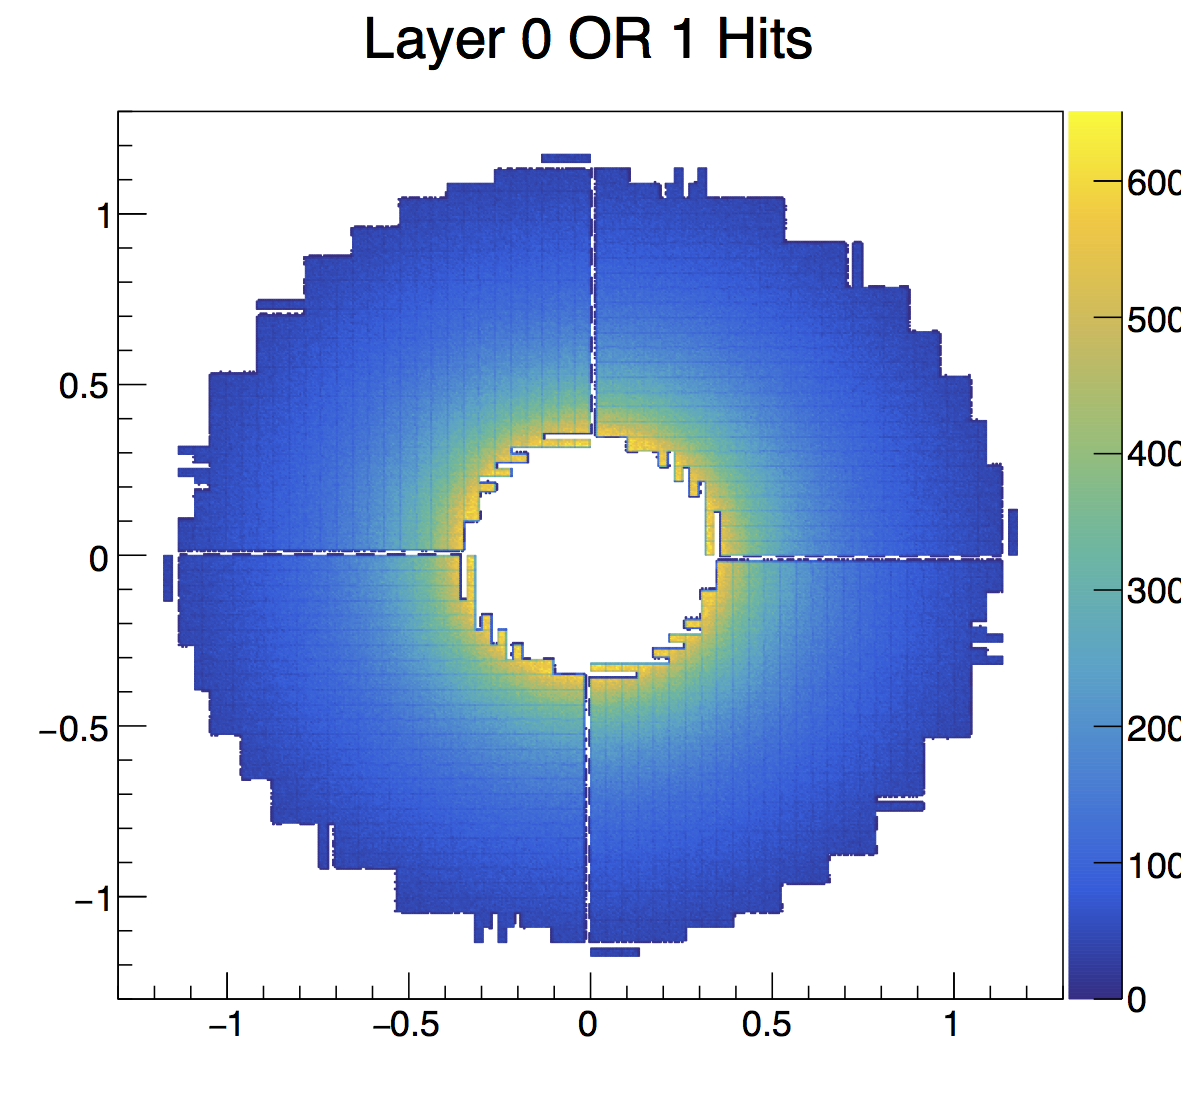
\includegraphics[width=.25\linewidth]{Dissertation/fig/LayerHits01-1190mm.png}
}
\end{center}
\caption{Efficiency plots produced using simulation data for the ETL with a 1190mm outer radius and 315mm inner radius following the Topolino design.}
\label{fig:chronoplots}
\end{figure}

\end{subsection}
\end{section}

%=== Chapter 3  ============================================
\chapter{Search for Anomolous Higgs to Vector-Meson Couplings}
\begin{section}{Motivation}

\cite{Maldacena:1997re,joesbook}. Figure \ref{fig:label}.

\end{section}

\begin{section}{Analysis Methods}
\begin{subsection}{Data}
The analysis begins with data based on a sample of proton-proton collisions collected by the Compact Muon Solenoid (CMS) detector in the LHC. ``Interesting'' events are selected by the first level of the CMS trigger system which uses information from the detector's calorimeters and muon detectors to select events for analysis in a fixed time interval of less than 4 $\mu s$. These events are then further processed by a high-level trigger processor farm, which decreases the event rate from around 100 kHz to less than 1 kHz, before the data is stored. Finally, the particle-flow algorithm reconstructs and identifies all particles from the events selected by the CMS trigger system. With the data properly processed and promptly reconstructed ``online,'' further analysis can be carried out ``offline.''
\end{subsection}
\begin{subsection}{Monte Carlo}
The analysis begins with data based on a sample of proton-proton collisions collected by the Compact Muon Solenoid (CMS) detector in the LHC. ``Interesting'' events are selected by the first level of the CMS trigger system which uses information from the detector's calorimeters and muon detectors to select events for analysis in a fixed time interval of less than 4 $\mu s$. These events are then further processed by a high-level trigger processor farm, which decreases the event rate from around 100 kHz to less than 1 kHz, before the data is stored. Finally, the particle-flow algorithm reconstructs and identifies all particles from the events selected by the CMS trigger system. With the data properly processed and promptly reconstructed ``online,'' further analysis can be carried out ``offline.''
\end{subsection}
\end{section}

\begin{section}{Results}

\end{section}

\appendix

\dsp

\chapter{The Compact Muon Solenoid}{\label{appendix:a}}
\begin{section}{The Detector}

The Compact Muon Solenoid (CMS) is a general purpose detector at the LHC, meaning it probes for the existence of a variety of new physics. The detector's namesake is a ``compact'' solenoid, the largest superconducting magnet ever built (with a length of 15m and diameter of 7m\cite{CMS:1994hea}), that generates a 4T magnetic field - strong enough to pull many high-energy, charged particles produced in a proton-proton collision towards CMS's detector layers. Particles first encounter the tracker, which is composed of several layers of silicon pixels and strip detectors. Essentially, a through-going particle leaves a cascading charge deposit that can be measured as an electrical signal. This results in an accurate measurement of the particle's position as it passes through various sections of the tracker, which can then be reconstructed to give the particle's entire trajectory. Track information provides fundamental insights like the charge and momentum of a particle, for instance, which can be inferred from the curvature of the particle's trajectory. Having passed through the tracker, particles then encounter the calorimeters, which will measure the final energies of emergent particles when possible. Energies of particles that interact by the electromagnetic force, electrons and photons, are measured by the Electromagnetic Calorimeter (ECAL) while those that interact by the strong force, hadrons, are measured by the Hadronic Calorimeter (HCAL). Finally, particles that escape the ECAL and HCAL -- now only muons and weakly interacting particles -- encounter the muon layer, where muons are tracked further, before leaving the bounds of CMS. The presence of neutrinos, which mostly pass through the detector undisturbed, and possibly yet-undiscovered particles can only be inferred. Conservation of momentum is key here: invisible particles will show up as missing energy in comparing the sum of the measured particle momenta to the overall energy of the collision.

\begin{figure}[htb]
\begin{center}
\subfloat[Sectional visualization of CMS.]      {
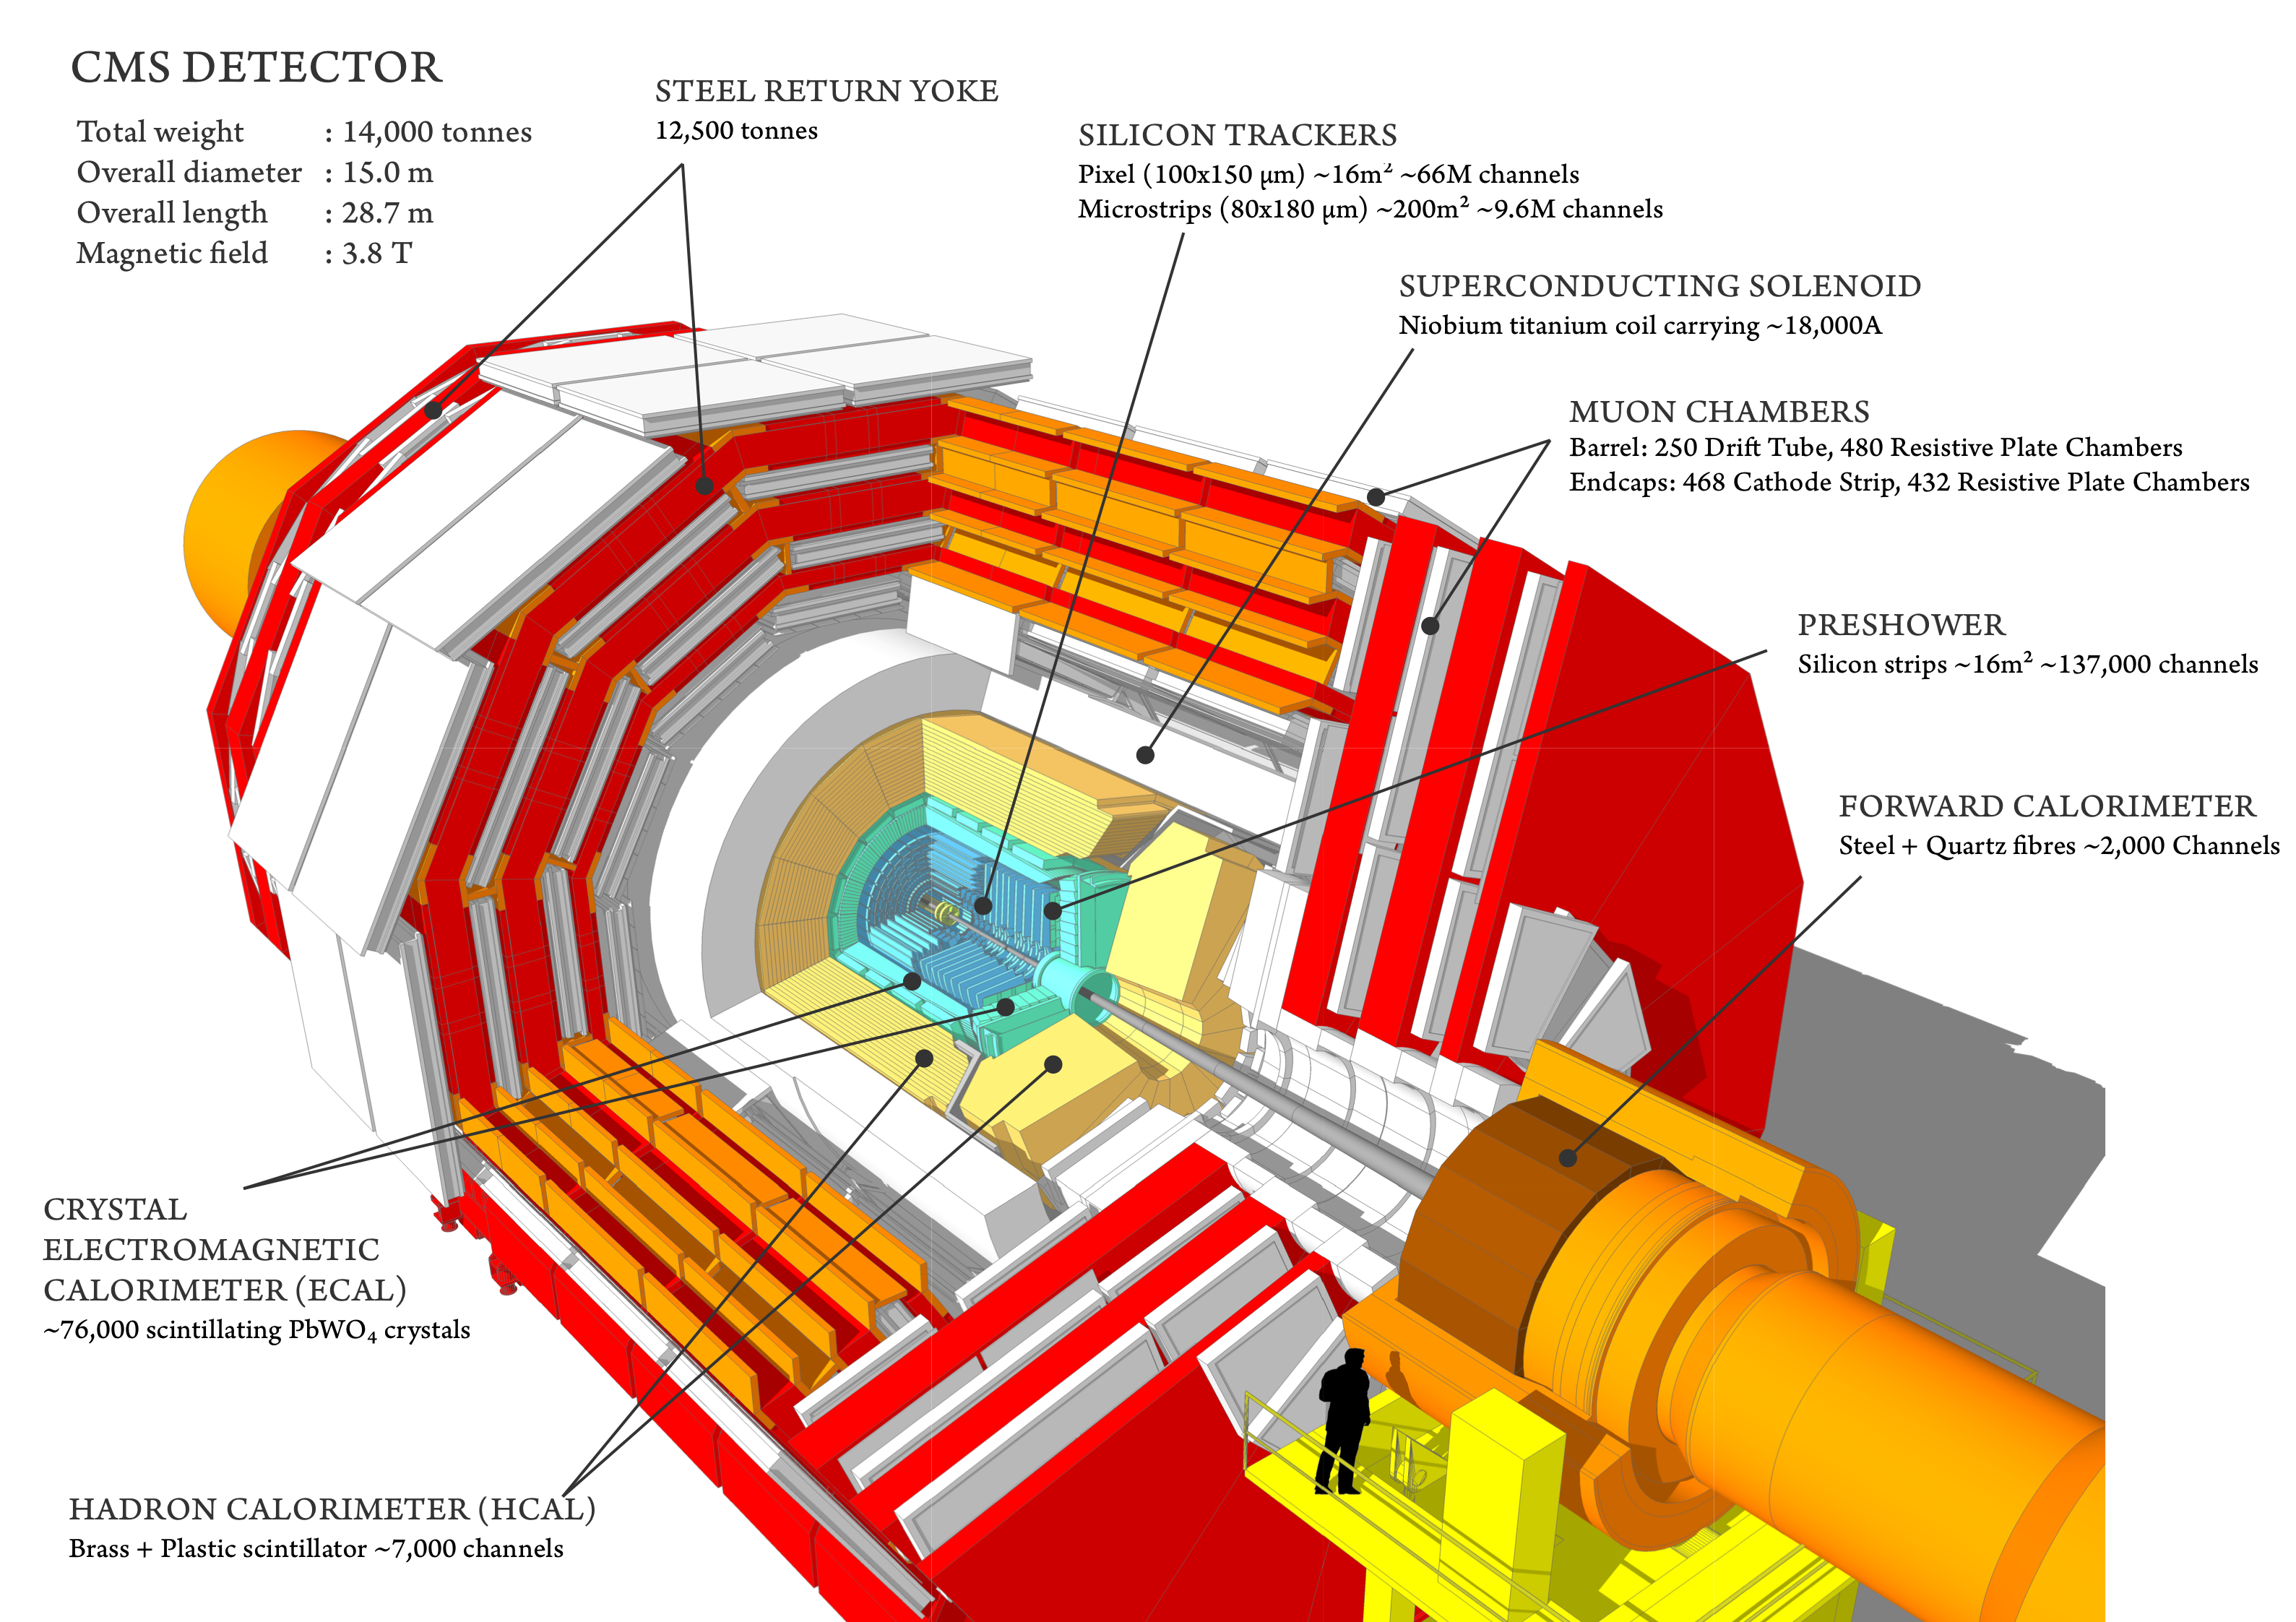
\includegraphics[width=.45\linewidth]{Dissertation/fig/cms-xsec.png}
}\quad
\subfloat[Cross section of detector showing various particle behavior.]      {
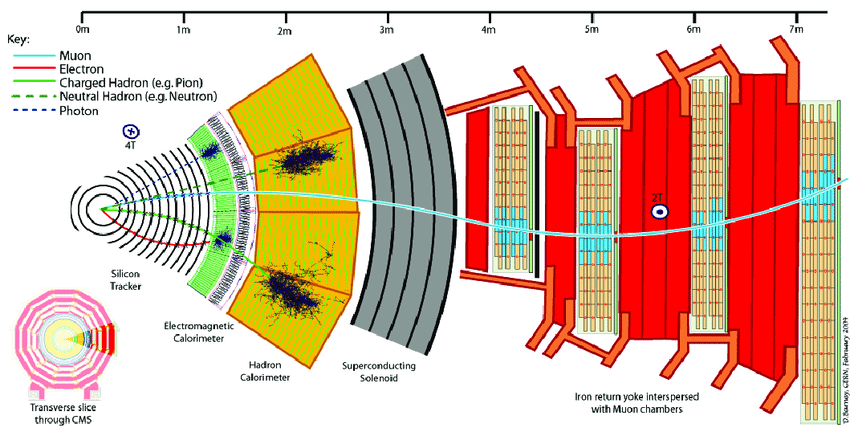
\includegraphics[width=.45\linewidth]{Dissertation/fig/cms-slice.png}
}
\end{center}
\caption{Visualizations of the design and function of CMS.}
\label{fig:cms-xsec}
\end{figure}

\end{section}
\begin{section}{CMS Coordinate System}

In the CMS Coordinate system, the $z$-axis is aligned along the beampipe, therefore running parallel to the barrel and perpendicular to the endcap of the detector. The $x$-axis points radially towards the center of the LHC, and the y-axis points orthogonal to $x$ and $z$. The azimuthal angle $\phi$ is defined about the $z$-axis, as in cylindrical coordinates, and the pseudo-rapidity $\eta$ is defined as

\begin{equation}
    \eta \equiv -\ln{\bigg[ \tan{\bigg( \frac{\theta}{2} \bigg)} \bigg]}
\end{equation}

\noindent where $\theta$ is the angle between the particle three-momentum and positive $z$-axis. See Figure \ref{fig:cms-coords} for a visualization of this coordinate system.

\begin{figure}[htb]
\begin{center}
\tdplotsetmaincoords{75}{50} % to reset previous setting
\begin{tikzpicture}[scale=2.7,tdplot_main_coords,rotate around x=90]
 
  % variables
  \def\rvec{1.2}
  \def\thetavec{40}
  \def\phivec{70}
  \def\R{1.1}
  \def\w{0.3}
 
  % axes
  \coordinate (O) at (0,0,0);
  \draw[thick,->] (0,0,0) -- (1,0,0) node[below left]{$x$};
  \draw[thick,->] (0,0,0) -- (0,1,0) node[below right]{$y$};
  \draw[thick,->] (0,0,0) -- (0,0,1) node[below right]{$z$};
  \tdplotsetcoord{P}{\rvec}{\thetavec}{\phivec}
 
  % vectors
  \draw[->,red] (O) -- (P) node[above left] {$P$};
  \draw[dashed,red] (O)  -- (Pxy);
  \draw[dashed,red] (P)  -- (Pxy);
  \draw[dashed,red] (Py) -- (Pxy);
 
  % circle - LHC
  \tdplotdrawarc[thick,rotate around x=90,black!70!blue]{(\R,0,0)}{\R}{0}{360}{}{}
 
  % compass - the line between CMS and ATLAS has a ~12° declination (http://googlecompass.com)
  \begin{scope}[shift={(1.1*\R,0,1.65*\R)},rotate around y=12]
    \draw[<->,black!50] (-\w,0,0) -- (\w,0,0);
    \draw[<->,black!50] (0,0,-\w) -- (0,0,\w);
    \node[above left,black!50,scale=0.6] at (-\w,0,0) {N};
  \end{scope}
 
  % nodes
  \node[left,align=center] at (0,0,1.1) {Jura};
  \node[right] at (\R,0,0) {LHC};
  \fill[radius=0.8pt,black!20!red]
    (O) circle node[left=4pt,below=2pt] {CMS};
  \draw[thick] (0.02,0,0) -- (0.5,0,0); % partially overdraw x-axis and CMS point
  \fill[radius=0.8pt,black!20!blue]
    (2*\R,0,0) circle
    node[right=4pt,below=2pt,scale=0.9] {ATLAS};
  \fill[radius=0.8pt,black!10!orange]
    ({\R*sqrt(2)/2+\R},0,{ \R*sqrt(2)/2}) circle % 45 degrees from ATLAS
    node[left=2pt,below=2pt,scale=0.8] {ALICE};
  \fill[radius=0.8pt,black!60!green]
    ({\R*sqrt(2)/2+\R},0,{-\R*sqrt(2)/2}) circle % 45 degrees from ATLAS
    node[below=2pt,right=2pt,scale=0.8] {LHCb};
 
  % arcs
  \tdplotdrawarc[->]{(O)}{0.2}{0}{\phivec}
    {above=2pt,right=-1pt,anchor=mid west}{$\phi$}
  \tdplotdrawarc[->,rotate around z=\phivec-90,rotate around y=-90]{(0,0,0)}{0.5}{0}{\thetavec}
    {anchor=mid east}{$\eta$}
 
\end{tikzpicture}
\end{center}
\caption{Diagram of CMS coordinate system.}
\label{fig:cms-coords}
\end{figure}

\end{section}
\end{mainmatter}

%----- Bibliography ----------------
\ssp
\bibliographystyle{JHEP3}
\bibliography{dissertation}

\end{document} 
